\chapter[Mathematica Code]{Mathematica Code}

The following Appendix contains the Wolfram Mathematica notebook file used to generate the data in Chapter~4. This code has been inserted into this document. All code is available at https://github.com/jsidabras/.

\subsection*{Definitions}

The following calculations and processes are performed:

\begin{enumerate}
    \item Solve the linear equation for the current and voltage relationships.
    \begin{itemize}
        \item \textbf{EqnMatrix}: This matrix is the mesh current relationship defined by the circuit
        \item \textbf{VVector}: This vector is the voltage relationship defined by the circuit
        \item \textbf{LinearSolve} and \textbf{FullSimplify}: Solve the linear equation $m\cdot X=b$ and plug it into the relationship for Z$_{\mathbf{21}}$ ``Open-circuit forward transimpedance''
        \item \textbf{Z$_{\mathbf{21}}$a}: Define the ``Open-circuit forward transimpedance'' as a function with inputs of the transmission line (inductance LL, capacitance CL), resonator (inductance LR, capacitance CR, resistance RR), and coupling coefficients (mutual capacitance kc and mutual inductance kL) at the frequency of $\Omega$.
    \end{itemize}
    \item Define the characteristics of the transmission-line circuit, resonator, and ``signal''.
    \item Solve \textbf{Z$_{\mathbf{21}}$a} over the frequency range of 255 to 700~GHz (8.51 to 23.35~cm$^{-1}$) and step the resonance shift between 2.0 to 1.0, which corresponds to resonance frequency shift to mimic the shift in static magnetic field.
    \begin{itemize}
        \item \textbf{Coupled Only}: Set the resonance of the bulk transmission-line to zero (gL) and solve for \textbf{Z$_{\mathbf{21}}$a} if only the resonator is coupled to the spins.
        \item \textbf{With Transmission}: Solve for \textbf{Z$_{\mathbf{21}}$a} if with both the transmission-line and the resonator coupled to the spins.
        \item \textbf{Only Transmission}: Solve for \textbf{Z$_{\mathbf{21}}$a} if with the transmission-line coupled to the spins and the resonator coupling set to zero (mutual capacitance kkc).
    \end{itemize}
    \item Solve and plot the frequency splittings generated for strong (100 time larger gR) and weak coupling regimes.
\end{enumerate}
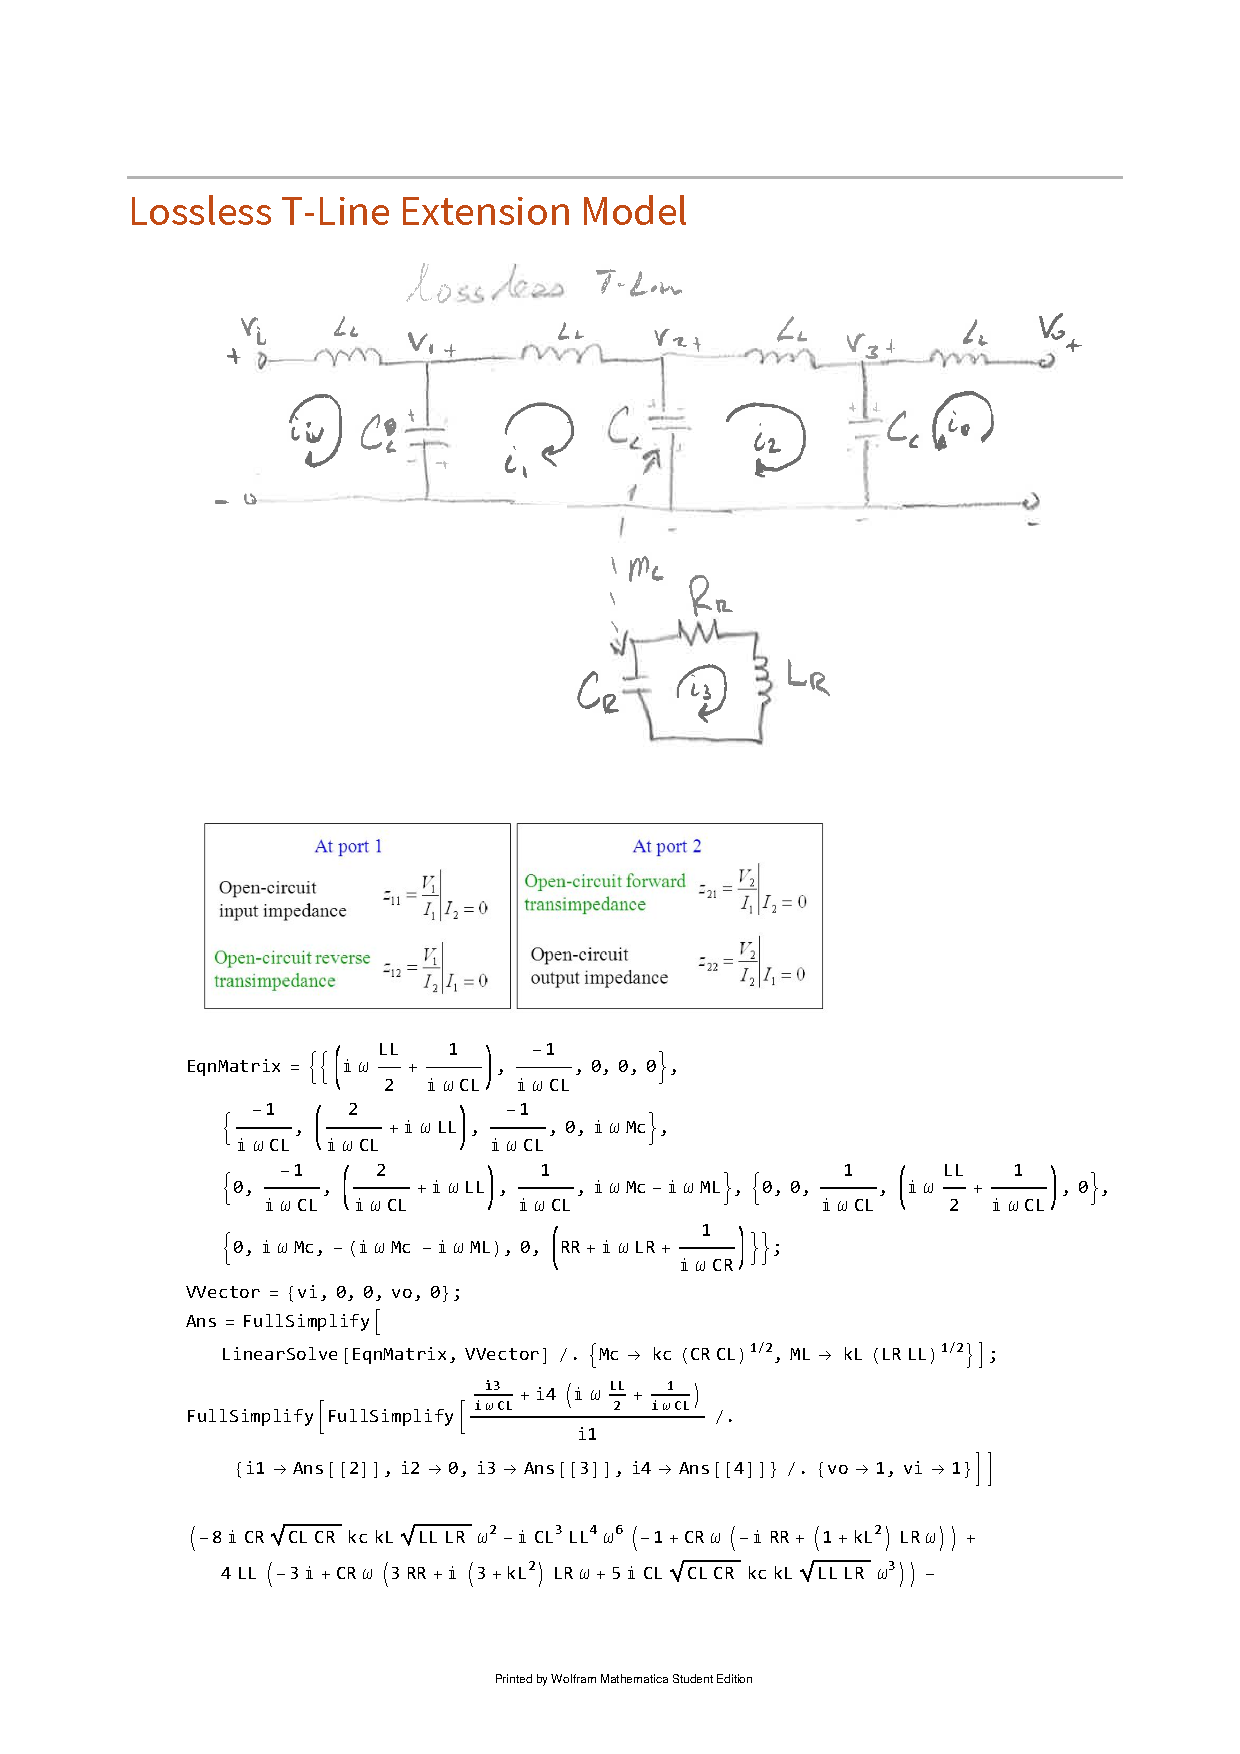
\includepdf[pages=-]{Kapitel/Appendix/MathematicaTHzWave.pdf}